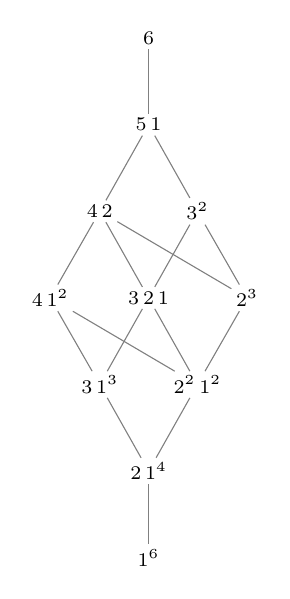
\begin{tikzpicture}[every node/.style={font=\scriptsize,inner sep=1.5pt}]
  \node (p6) at (0.00,6.60) {$6$};
  \node (p5_1) at (0.00,5.50) {$5\,1$};
  \node (p4_2) at (-0.62,4.40) {$4\,2$};
  \node (p4_1_1) at (-1.25,3.30) {$4\,1^{2}$};
  \node (p3_3) at (0.62,4.40) {$3^{2}$};
  \node (p3_2_1) at (0.00,3.30) {$3\,2\,1$};
  \node (p3_1_1_1) at (-0.62,2.20) {$3\,1^{3}$};
  \node (p2_2_2) at (1.25,3.30) {$2^{3}$};
  \node (p2_2_1_1) at (0.62,2.20) {$2^{2}\,1^{2}$};
  \node (p2_1_1_1_1) at (0.00,1.10) {$2\,1^{4}$};
  \node (p1_1_1_1_1_1) at (0.00,0.00) {$1^{6}$};
  \draw[gray] (p2_1_1_1_1) -- (p1_1_1_1_1_1);
  \draw[gray] (p2_2_1_1) -- (p2_1_1_1_1);
  \draw[gray] (p2_2_2) -- (p2_2_1_1);
  \draw[gray] (p3_1_1_1) -- (p2_1_1_1_1);
  \draw[gray] (p3_2_1) -- (p2_2_1_1);
  \draw[gray] (p3_2_1) -- (p3_1_1_1);
  \draw[gray] (p3_3) -- (p2_2_2);
  \draw[gray] (p3_3) -- (p3_2_1);
  \draw[gray] (p4_1_1) -- (p2_2_1_1);
  \draw[gray] (p4_1_1) -- (p3_1_1_1);
  \draw[gray] (p4_2) -- (p2_2_2);
  \draw[gray] (p4_2) -- (p3_2_1);
  \draw[gray] (p4_2) -- (p4_1_1);
  \draw[gray] (p5_1) -- (p3_3);
  \draw[gray] (p5_1) -- (p4_2);
  \draw[gray] (p6) -- (p5_1);
\end{tikzpicture}
